In this chapter I present some of the results obtained from performing experiments with the
simulation application described in the last three chapters.

\section{Quantitative evaluation}
\subsection{Simulation accuracy}
The quality of simulation results is hard to measure quantitatively, since simulation is usually
employed to calculate the behaviour of systems whose exact solution is not known. Therefore it is
useful to run the simulation on a system which can be characterized analytically, and to compare
the results against the theoretical values.

For this comparison I chose to simulate a \emph{gyroscope} (figure~\ref{gyroscope}). It consists
of a single rotating rigid body and a `nail' constraint (appendix~\ref{constrNail}) holding one
end of its axis in place. When gravity acts on the centre of mass of the body, the `nail' exerts
a balancing force and a torque which stop the gyroscope from falling down and causes forced
precession. The angular velocity of precession can be derived analytically~\cite{Julian:notes}
and depends only on the gravitational force, the distance between the centre of mass and the
nail, and the angular momentum of the body.

\begin{figure}
\centerline{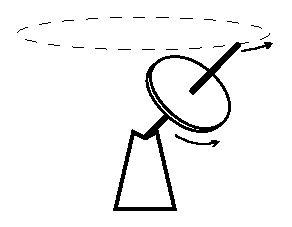
\includegraphics{figures/gyroscope}}
\caption{Schematic drawing of a gyroscope. The disc rapidly rotates about its own axis, and
    gravity causes a slower precession movement about the vertical axis (shown as a dotted line).
    \label{gyroscope}}
\end{figure}

I set up the initial conditions for the simulation to reflect values one might find in an actual
toy gyroscope (20 revolutions per second about the gyroscope axis, one full circle of precession
in 8 seconds). I then ran the simulation for 8~s, using an average time step length of about
$2.3\cdot 10^{-4}$~s. The simulation performed one full circle of precession in 7.953~s, which
is within 0.6~\% of the theoretical value. Over the course of 8~s, the body rotated by $320.36\pi$
radians about its own axis (160.18 revolutions), which differs from the theoretical value by only
0.1~\%. These errors varied very little even in simulations using larger time steps.
The effects of nutation~\cite{Feynman:63} were small for the chosen initial conditions but may
have contributed towards the errors.

These results are very encouraging, but is interesting to also observe a different error, namely
the amount by which the constraint drifts apart. Usually this drift is compensated in the Lagrange
multiplier method so that it never manifests itself, but temporarily deactivating this
correction\footnote{by setting $k=d=0$ in equation~\ref{lagrangeEquation}.} makes the error
introduced by the ODE solver observable.

\begin{figure}
\centerline{% GNUPLOT: LaTeX picture with Postscript
\begingroup%
  \makeatletter%
  \newcommand{\GNUPLOTspecial}{%
    \@sanitize\catcode`\%=14\relax\special}%
  \setlength{\unitlength}{0.1bp}%
\begin{picture}(3600,2160)(0,0)%
{\GNUPLOTspecial{"
%!PS-Adobe-2.0 EPSF-2.0
%%Title: errorplot.tex
%%Creator: gnuplot 4.0 patchlevel 0
%%CreationDate: Mon Apr 17 12:02:25 2006
%%DocumentFonts: 
%%BoundingBox: 0 0 360 216
%%Orientation: Landscape
%%EndComments
/gnudict 256 dict def
gnudict begin
/Color false def
/Solid false def
/gnulinewidth 5.000 def
/userlinewidth gnulinewidth def
/vshift -33 def
/dl {10.0 mul} def
/hpt_ 31.5 def
/vpt_ 31.5 def
/hpt hpt_ def
/vpt vpt_ def
/Rounded false def
/M {moveto} bind def
/L {lineto} bind def
/R {rmoveto} bind def
/V {rlineto} bind def
/N {newpath moveto} bind def
/C {setrgbcolor} bind def
/f {rlineto fill} bind def
/vpt2 vpt 2 mul def
/hpt2 hpt 2 mul def
/Lshow { currentpoint stroke M
  0 vshift R show } def
/Rshow { currentpoint stroke M
  dup stringwidth pop neg vshift R show } def
/Cshow { currentpoint stroke M
  dup stringwidth pop -2 div vshift R show } def
/UP { dup vpt_ mul /vpt exch def hpt_ mul /hpt exch def
  /hpt2 hpt 2 mul def /vpt2 vpt 2 mul def } def
/DL { Color {setrgbcolor Solid {pop []} if 0 setdash }
 {pop pop pop 0 setgray Solid {pop []} if 0 setdash} ifelse } def
/BL { stroke userlinewidth 2 mul setlinewidth
      Rounded { 1 setlinejoin 1 setlinecap } if } def
/AL { stroke userlinewidth 2 div setlinewidth
      Rounded { 1 setlinejoin 1 setlinecap } if } def
/UL { dup gnulinewidth mul /userlinewidth exch def
      dup 1 lt {pop 1} if 10 mul /udl exch def } def
/PL { stroke userlinewidth setlinewidth
      Rounded { 1 setlinejoin 1 setlinecap } if } def
/LTw { PL [] 1 setgray } def
/LTb { BL [] 0 0 0 DL } def
/LTa { AL [1 udl mul 2 udl mul] 0 setdash 0 0 0 setrgbcolor } def
/LT0 { PL [] 1 0 0 DL } def
/LT1 { PL [4 dl 2 dl] 0 1 0 DL } def
/LT2 { PL [2 dl 3 dl] 0 0 1 DL } def
/LT3 { PL [1 dl 1.5 dl] 1 0 1 DL } def
/LT4 { PL [5 dl 2 dl 1 dl 2 dl] 0 1 1 DL } def
/LT5 { PL [4 dl 3 dl 1 dl 3 dl] 1 1 0 DL } def
/LT6 { PL [2 dl 2 dl 2 dl 4 dl] 0 0 0 DL } def
/LT7 { PL [2 dl 2 dl 2 dl 2 dl 2 dl 4 dl] 1 0.3 0 DL } def
/LT8 { PL [2 dl 2 dl 2 dl 2 dl 2 dl 2 dl 2 dl 4 dl] 0.5 0.5 0.5 DL } def
/Pnt { stroke [] 0 setdash
   gsave 1 setlinecap M 0 0 V stroke grestore } def
/Dia { stroke [] 0 setdash 2 copy vpt add M
  hpt neg vpt neg V hpt vpt neg V
  hpt vpt V hpt neg vpt V closepath stroke
  Pnt } def
/Pls { stroke [] 0 setdash vpt sub M 0 vpt2 V
  currentpoint stroke M
  hpt neg vpt neg R hpt2 0 V stroke
  } def
/Box { stroke [] 0 setdash 2 copy exch hpt sub exch vpt add M
  0 vpt2 neg V hpt2 0 V 0 vpt2 V
  hpt2 neg 0 V closepath stroke
  Pnt } def
/Crs { stroke [] 0 setdash exch hpt sub exch vpt add M
  hpt2 vpt2 neg V currentpoint stroke M
  hpt2 neg 0 R hpt2 vpt2 V stroke } def
/TriU { stroke [] 0 setdash 2 copy vpt 1.12 mul add M
  hpt neg vpt -1.62 mul V
  hpt 2 mul 0 V
  hpt neg vpt 1.62 mul V closepath stroke
  Pnt  } def
/Star { 2 copy Pls Crs } def
/BoxF { stroke [] 0 setdash exch hpt sub exch vpt add M
  0 vpt2 neg V  hpt2 0 V  0 vpt2 V
  hpt2 neg 0 V  closepath fill } def
/TriUF { stroke [] 0 setdash vpt 1.12 mul add M
  hpt neg vpt -1.62 mul V
  hpt 2 mul 0 V
  hpt neg vpt 1.62 mul V closepath fill } def
/TriD { stroke [] 0 setdash 2 copy vpt 1.12 mul sub M
  hpt neg vpt 1.62 mul V
  hpt 2 mul 0 V
  hpt neg vpt -1.62 mul V closepath stroke
  Pnt  } def
/TriDF { stroke [] 0 setdash vpt 1.12 mul sub M
  hpt neg vpt 1.62 mul V
  hpt 2 mul 0 V
  hpt neg vpt -1.62 mul V closepath fill} def
/DiaF { stroke [] 0 setdash vpt add M
  hpt neg vpt neg V hpt vpt neg V
  hpt vpt V hpt neg vpt V closepath fill } def
/Pent { stroke [] 0 setdash 2 copy gsave
  translate 0 hpt M 4 {72 rotate 0 hpt L} repeat
  closepath stroke grestore Pnt } def
/PentF { stroke [] 0 setdash gsave
  translate 0 hpt M 4 {72 rotate 0 hpt L} repeat
  closepath fill grestore } def
/Circle { stroke [] 0 setdash 2 copy
  hpt 0 360 arc stroke Pnt } def
/CircleF { stroke [] 0 setdash hpt 0 360 arc fill } def
/C0 { BL [] 0 setdash 2 copy moveto vpt 90 450  arc } bind def
/C1 { BL [] 0 setdash 2 copy        moveto
       2 copy  vpt 0 90 arc closepath fill
               vpt 0 360 arc closepath } bind def
/C2 { BL [] 0 setdash 2 copy moveto
       2 copy  vpt 90 180 arc closepath fill
               vpt 0 360 arc closepath } bind def
/C3 { BL [] 0 setdash 2 copy moveto
       2 copy  vpt 0 180 arc closepath fill
               vpt 0 360 arc closepath } bind def
/C4 { BL [] 0 setdash 2 copy moveto
       2 copy  vpt 180 270 arc closepath fill
               vpt 0 360 arc closepath } bind def
/C5 { BL [] 0 setdash 2 copy moveto
       2 copy  vpt 0 90 arc
       2 copy moveto
       2 copy  vpt 180 270 arc closepath fill
               vpt 0 360 arc } bind def
/C6 { BL [] 0 setdash 2 copy moveto
      2 copy  vpt 90 270 arc closepath fill
              vpt 0 360 arc closepath } bind def
/C7 { BL [] 0 setdash 2 copy moveto
      2 copy  vpt 0 270 arc closepath fill
              vpt 0 360 arc closepath } bind def
/C8 { BL [] 0 setdash 2 copy moveto
      2 copy vpt 270 360 arc closepath fill
              vpt 0 360 arc closepath } bind def
/C9 { BL [] 0 setdash 2 copy moveto
      2 copy  vpt 270 450 arc closepath fill
              vpt 0 360 arc closepath } bind def
/C10 { BL [] 0 setdash 2 copy 2 copy moveto vpt 270 360 arc closepath fill
       2 copy moveto
       2 copy vpt 90 180 arc closepath fill
               vpt 0 360 arc closepath } bind def
/C11 { BL [] 0 setdash 2 copy moveto
       2 copy  vpt 0 180 arc closepath fill
       2 copy moveto
       2 copy  vpt 270 360 arc closepath fill
               vpt 0 360 arc closepath } bind def
/C12 { BL [] 0 setdash 2 copy moveto
       2 copy  vpt 180 360 arc closepath fill
               vpt 0 360 arc closepath } bind def
/C13 { BL [] 0 setdash  2 copy moveto
       2 copy  vpt 0 90 arc closepath fill
       2 copy moveto
       2 copy  vpt 180 360 arc closepath fill
               vpt 0 360 arc closepath } bind def
/C14 { BL [] 0 setdash 2 copy moveto
       2 copy  vpt 90 360 arc closepath fill
               vpt 0 360 arc } bind def
/C15 { BL [] 0 setdash 2 copy vpt 0 360 arc closepath fill
               vpt 0 360 arc closepath } bind def
/Rec   { newpath 4 2 roll moveto 1 index 0 rlineto 0 exch rlineto
       neg 0 rlineto closepath } bind def
/Square { dup Rec } bind def
/Bsquare { vpt sub exch vpt sub exch vpt2 Square } bind def
/S0 { BL [] 0 setdash 2 copy moveto 0 vpt rlineto BL Bsquare } bind def
/S1 { BL [] 0 setdash 2 copy vpt Square fill Bsquare } bind def
/S2 { BL [] 0 setdash 2 copy exch vpt sub exch vpt Square fill Bsquare } bind def
/S3 { BL [] 0 setdash 2 copy exch vpt sub exch vpt2 vpt Rec fill Bsquare } bind def
/S4 { BL [] 0 setdash 2 copy exch vpt sub exch vpt sub vpt Square fill Bsquare } bind def
/S5 { BL [] 0 setdash 2 copy 2 copy vpt Square fill
       exch vpt sub exch vpt sub vpt Square fill Bsquare } bind def
/S6 { BL [] 0 setdash 2 copy exch vpt sub exch vpt sub vpt vpt2 Rec fill Bsquare } bind def
/S7 { BL [] 0 setdash 2 copy exch vpt sub exch vpt sub vpt vpt2 Rec fill
       2 copy vpt Square fill
       Bsquare } bind def
/S8 { BL [] 0 setdash 2 copy vpt sub vpt Square fill Bsquare } bind def
/S9 { BL [] 0 setdash 2 copy vpt sub vpt vpt2 Rec fill Bsquare } bind def
/S10 { BL [] 0 setdash 2 copy vpt sub vpt Square fill 2 copy exch vpt sub exch vpt Square fill
       Bsquare } bind def
/S11 { BL [] 0 setdash 2 copy vpt sub vpt Square fill 2 copy exch vpt sub exch vpt2 vpt Rec fill
       Bsquare } bind def
/S12 { BL [] 0 setdash 2 copy exch vpt sub exch vpt sub vpt2 vpt Rec fill Bsquare } bind def
/S13 { BL [] 0 setdash 2 copy exch vpt sub exch vpt sub vpt2 vpt Rec fill
       2 copy vpt Square fill Bsquare } bind def
/S14 { BL [] 0 setdash 2 copy exch vpt sub exch vpt sub vpt2 vpt Rec fill
       2 copy exch vpt sub exch vpt Square fill Bsquare } bind def
/S15 { BL [] 0 setdash 2 copy Bsquare fill Bsquare } bind def
/D0 { gsave translate 45 rotate 0 0 S0 stroke grestore } bind def
/D1 { gsave translate 45 rotate 0 0 S1 stroke grestore } bind def
/D2 { gsave translate 45 rotate 0 0 S2 stroke grestore } bind def
/D3 { gsave translate 45 rotate 0 0 S3 stroke grestore } bind def
/D4 { gsave translate 45 rotate 0 0 S4 stroke grestore } bind def
/D5 { gsave translate 45 rotate 0 0 S5 stroke grestore } bind def
/D6 { gsave translate 45 rotate 0 0 S6 stroke grestore } bind def
/D7 { gsave translate 45 rotate 0 0 S7 stroke grestore } bind def
/D8 { gsave translate 45 rotate 0 0 S8 stroke grestore } bind def
/D9 { gsave translate 45 rotate 0 0 S9 stroke grestore } bind def
/D10 { gsave translate 45 rotate 0 0 S10 stroke grestore } bind def
/D11 { gsave translate 45 rotate 0 0 S11 stroke grestore } bind def
/D12 { gsave translate 45 rotate 0 0 S12 stroke grestore } bind def
/D13 { gsave translate 45 rotate 0 0 S13 stroke grestore } bind def
/D14 { gsave translate 45 rotate 0 0 S14 stroke grestore } bind def
/D15 { gsave translate 45 rotate 0 0 S15 stroke grestore } bind def
/DiaE { stroke [] 0 setdash vpt add M
  hpt neg vpt neg V hpt vpt neg V
  hpt vpt V hpt neg vpt V closepath stroke } def
/BoxE { stroke [] 0 setdash exch hpt sub exch vpt add M
  0 vpt2 neg V hpt2 0 V 0 vpt2 V
  hpt2 neg 0 V closepath stroke } def
/TriUE { stroke [] 0 setdash vpt 1.12 mul add M
  hpt neg vpt -1.62 mul V
  hpt 2 mul 0 V
  hpt neg vpt 1.62 mul V closepath stroke } def
/TriDE { stroke [] 0 setdash vpt 1.12 mul sub M
  hpt neg vpt 1.62 mul V
  hpt 2 mul 0 V
  hpt neg vpt -1.62 mul V closepath stroke } def
/PentE { stroke [] 0 setdash gsave
  translate 0 hpt M 4 {72 rotate 0 hpt L} repeat
  closepath stroke grestore } def
/CircE { stroke [] 0 setdash 
  hpt 0 360 arc stroke } def
/Opaque { gsave closepath 1 setgray fill grestore 0 setgray closepath } def
/DiaW { stroke [] 0 setdash vpt add M
  hpt neg vpt neg V hpt vpt neg V
  hpt vpt V hpt neg vpt V Opaque stroke } def
/BoxW { stroke [] 0 setdash exch hpt sub exch vpt add M
  0 vpt2 neg V hpt2 0 V 0 vpt2 V
  hpt2 neg 0 V Opaque stroke } def
/TriUW { stroke [] 0 setdash vpt 1.12 mul add M
  hpt neg vpt -1.62 mul V
  hpt 2 mul 0 V
  hpt neg vpt 1.62 mul V Opaque stroke } def
/TriDW { stroke [] 0 setdash vpt 1.12 mul sub M
  hpt neg vpt 1.62 mul V
  hpt 2 mul 0 V
  hpt neg vpt -1.62 mul V Opaque stroke } def
/PentW { stroke [] 0 setdash gsave
  translate 0 hpt M 4 {72 rotate 0 hpt L} repeat
  Opaque stroke grestore } def
/CircW { stroke [] 0 setdash 
  hpt 0 360 arc Opaque stroke } def
/BoxFill { gsave Rec 1 setgray fill grestore } def
/BoxColFill {
  gsave Rec
  /Fillden exch def
  currentrgbcolor
  /ColB exch def /ColG exch def /ColR exch def
  /ColR ColR Fillden mul Fillden sub 1 add def
  /ColG ColG Fillden mul Fillden sub 1 add def
  /ColB ColB Fillden mul Fillden sub 1 add def
  ColR ColG ColB setrgbcolor
  fill grestore } def
%
% PostScript Level 1 Pattern Fill routine
% Usage: x y w h s a XX PatternFill
%	x,y = lower left corner of box to be filled
%	w,h = width and height of box
%	  a = angle in degrees between lines and x-axis
%	 XX = 0/1 for no/yes cross-hatch
%
/PatternFill { gsave /PFa [ 9 2 roll ] def
    PFa 0 get PFa 2 get 2 div add PFa 1 get PFa 3 get 2 div add translate
    PFa 2 get -2 div PFa 3 get -2 div PFa 2 get PFa 3 get Rec
    gsave 1 setgray fill grestore clip
    currentlinewidth 0.5 mul setlinewidth
    /PFs PFa 2 get dup mul PFa 3 get dup mul add sqrt def
    0 0 M PFa 5 get rotate PFs -2 div dup translate
	0 1 PFs PFa 4 get div 1 add floor cvi
	{ PFa 4 get mul 0 M 0 PFs V } for
    0 PFa 6 get ne {
	0 1 PFs PFa 4 get div 1 add floor cvi
	{ PFa 4 get mul 0 2 1 roll M PFs 0 V } for
    } if
    stroke grestore } def
%
/Symbol-Oblique /Symbol findfont [1 0 .167 1 0 0] makefont
dup length dict begin {1 index /FID eq {pop pop} {def} ifelse} forall
currentdict end definefont pop
end
%%EndProlog
gnudict begin
gsave
0 0 translate
0.100 0.100 scale
0 setgray
newpath
1.000 UL
LTb
550 300 M
31 0 V
1821 0 R
-31 0 V
550 393 M
63 0 V
1789 0 R
-63 0 V
1.000 UL
LTb
550 485 M
31 0 V
1821 0 R
-31 0 V
550 578 M
63 0 V
1789 0 R
-63 0 V
1.000 UL
LTb
550 671 M
31 0 V
1821 0 R
-31 0 V
550 763 M
63 0 V
1789 0 R
-63 0 V
1.000 UL
LTb
550 856 M
31 0 V
1821 0 R
-31 0 V
550 948 M
63 0 V
1789 0 R
-63 0 V
1.000 UL
LTb
550 1041 M
31 0 V
1821 0 R
-31 0 V
550 1134 M
63 0 V
1789 0 R
-63 0 V
1.000 UL
LTb
550 1226 M
31 0 V
1821 0 R
-31 0 V
550 1319 M
63 0 V
1789 0 R
-63 0 V
1.000 UL
LTb
550 1412 M
31 0 V
1821 0 R
-31 0 V
550 1504 M
63 0 V
1789 0 R
-63 0 V
1.000 UL
LTb
550 1597 M
31 0 V
1821 0 R
-31 0 V
550 1689 M
63 0 V
1789 0 R
-63 0 V
1.000 UL
LTb
550 1782 M
31 0 V
1821 0 R
-31 0 V
550 1875 M
63 0 V
1789 0 R
-63 0 V
1.000 UL
LTb
550 1967 M
31 0 V
1821 0 R
-31 0 V
550 2060 M
63 0 V
1789 0 R
-63 0 V
1.000 UL
LTb
550 300 M
0 63 V
0 1697 R
0 -63 V
1.000 UL
LTb
689 300 M
0 31 V
0 1729 R
0 -31 V
771 300 M
0 31 V
0 1729 R
0 -31 V
829 300 M
0 31 V
0 1729 R
0 -31 V
874 300 M
0 31 V
0 1729 R
0 -31 V
910 300 M
0 31 V
0 1729 R
0 -31 V
941 300 M
0 31 V
0 1729 R
0 -31 V
968 300 M
0 31 V
0 1729 R
0 -31 V
992 300 M
0 31 V
0 1729 R
0 -31 V
1013 300 M
0 63 V
0 1697 R
0 -63 V
1.000 UL
LTb
1152 300 M
0 31 V
0 1729 R
0 -31 V
1234 300 M
0 31 V
0 1729 R
0 -31 V
1292 300 M
0 31 V
0 1729 R
0 -31 V
1337 300 M
0 31 V
0 1729 R
0 -31 V
1373 300 M
0 31 V
0 1729 R
0 -31 V
1404 300 M
0 31 V
0 1729 R
0 -31 V
1431 300 M
0 31 V
0 1729 R
0 -31 V
1455 300 M
0 31 V
0 1729 R
0 -31 V
1476 300 M
0 63 V
0 1697 R
0 -63 V
1.000 UL
LTb
1615 300 M
0 31 V
0 1729 R
0 -31 V
1697 300 M
0 31 V
0 1729 R
0 -31 V
1755 300 M
0 31 V
0 1729 R
0 -31 V
1800 300 M
0 31 V
0 1729 R
0 -31 V
1836 300 M
0 31 V
0 1729 R
0 -31 V
1867 300 M
0 31 V
0 1729 R
0 -31 V
1894 300 M
0 31 V
0 1729 R
0 -31 V
1918 300 M
0 31 V
0 1729 R
0 -31 V
1939 300 M
0 63 V
0 1697 R
0 -63 V
1.000 UL
LTb
2078 300 M
0 31 V
0 1729 R
0 -31 V
2160 300 M
0 31 V
0 1729 R
0 -31 V
2218 300 M
0 31 V
0 1729 R
0 -31 V
2263 300 M
0 31 V
0 1729 R
0 -31 V
2299 300 M
0 31 V
0 1729 R
0 -31 V
2330 300 M
0 31 V
0 1729 R
0 -31 V
2357 300 M
0 31 V
0 1729 R
0 -31 V
2381 300 M
0 31 V
0 1729 R
0 -31 V
2402 300 M
0 63 V
0 1697 R
0 -63 V
1.000 UL
LTb
1.000 UL
LTb
550 300 M
1852 0 V
0 1760 V
-1852 0 V
550 300 L
LTb
LTb
1.000 UP
1.000 UP
1.000 UL
LT0
LTb
LT0
650 1869 M
263 0 V
1224 -87 R
-57 -93 V
-73 -92 V
-85 -93 V
-89 -92 V
-92 -93 V
-93 -93 V
-92 -92 V
-93 -93 V
-93 -93 V
-92 -92 V
-93 -93 V
-92 -92 V
-93 -93 V
908 485 L
815 393 L
2137 1782 Pls
2080 1689 Pls
2007 1597 Pls
1922 1504 Pls
1833 1412 Pls
1741 1319 Pls
1648 1226 Pls
1556 1134 Pls
1463 1041 Pls
1370 948 Pls
1278 856 Pls
1185 763 Pls
1093 671 Pls
1000 578 Pls
908 485 Pls
815 393 Pls
782 1869 Pls
1.000 UP
1.000 UL
LT1
LTb
LT1
650 1712 M
263 0 V
1224 285 R
-57 -146 V
-73 -94 V
-85 -94 V
-89 -91 V
-92 -93 V
-93 -93 V
-92 -91 V
-93 -37 V
-93 -65 V
-92 -71 V
-93 12 V
-92 -23 V
1000 995 L
-92 33 V
815 971 L
2137 1997 Crs
2080 1851 Crs
2007 1757 Crs
1922 1663 Crs
1833 1572 Crs
1741 1479 Crs
1648 1386 Crs
1556 1295 Crs
1463 1258 Crs
1370 1193 Crs
1278 1122 Crs
1185 1134 Crs
1093 1111 Crs
1000 995 Crs
908 1028 Crs
815 971 Crs
782 1712 Crs
1.000 UL
LTb
550 300 M
1852 0 V
0 1760 V
-1852 0 V
550 300 L
1.000 UP
stroke
grestore
end
showpage
}}%
\put(963,1712){\makebox(0,0)[l]{error over 8 sec}}%
\put(963,1869){\makebox(0,0)[l]{error per step}}%
\put(1476,50){\makebox(0,0){time step length}}%
\put(100,1180){%
\special{ps: gsave currentpoint currentpoint translate
270 rotate neg exch neg exch translate}%
\makebox(0,0)[b]{\shortstack{error}}%
\special{ps: currentpoint grestore moveto}%
}%
\put(2402,200){\makebox(0,0){ 0.1}}%
\put(1939,200){\makebox(0,0){ 0.01}}%
\put(1476,200){\makebox(0,0){ 0.001}}%
\put(1013,200){\makebox(0,0){ 1e-04}}%
\put(550,200){\makebox(0,0){ 1e-05}}%
\put(500,2060){\makebox(0,0)[r]{ 100}}%
\put(500,1875){\makebox(0,0)[r]{ 1}}%
\put(500,1689){\makebox(0,0)[r]{ 0.01}}%
\put(500,1504){\makebox(0,0)[r]{ 1e-04}}%
\put(500,1319){\makebox(0,0)[r]{ 1e-06}}%
\put(500,1134){\makebox(0,0)[r]{ 1e-08}}%
\put(500,948){\makebox(0,0)[r]{ 1e-10}}%
\put(500,763){\makebox(0,0)[r]{ 1e-12}}%
\put(500,578){\makebox(0,0)[r]{ 1e-14}}%
\put(500,393){\makebox(0,0)[r]{ 1e-16}}%
\end{picture}%
\endgroup
\endinput
}
\caption{Errors introduced by the ODE solver for different step sizes $h$.
    Solid line: target error (difference between $O(h^4)$ and $O(h^5)$ approximations) of
    the ODE solver. Dashed line: drift of `nail' constraint in gyroscope simulation after
    8~s simulation time.\label{errorplot}}
\end{figure}

Figure~\ref{errorplot} shows by what distance the gyroscope's `nail' constraint drifted apart
after 8~s of simulation time, for a wide range of different step sizes. Since I used the
adaptive-stepsize algorithm described in section~\ref{solvingODEs}, I actually set the target
error (solid line in figure~\ref{errorplot}) and then used the average step size taken by the
solver as abscissa. There are some noteworthy features about this plot:

\begin{itemize}
\item The logarithmic axes are scaled such that one order of magnitude in the horizontal has the
    same length as five orders of magnitude in the vertical. Observe that in this scaling, the
    solid line (error per time step) is an almost perfect straight line with gradient~1. This
    shows that the error is indeed an $O(h^5)$ function of the step size, as expected.
\item Over a wide range of step sizes, the plot of the total accumulated error is parallel to the
    solid line. This means the total error is also $O(h^5)$, which is in fact better than
    expected: although the approximation in each time step is $O(h^5)$, the number of steps
    required is inversely proportional to the step length, so one might expect a larger overall
    error. This relationship indicates that the ODE solver's target error can in fact be used
    as a reliable estimate of the overall error to within a constant factor.
\item As step sizes $h$ become very small~-- below about $3\cdot 10^{-4}$~s~-- the error in each
    step continues to scale order $O(h^5)$, but due to the huge number of steps, the accumulated
    error cannot be reduced much further. However, the errors here are in the range of nanometres,
    so they should be of little concern for computer graphics purposes.
\end{itemize}

In summary, the results for the simple gyroscope simulation inspire the confidence that the
implementation is reliable and will continue to produce realistic results for complicated systems
which lack an exact solution. They also show that the target error can conveniently be adjusted
to match the requirements, because more CPU time does~-- within sensible bounds~-- buy higher
accuracy.


\section{Qualitative evaluation}


\section{Limitations}
friction

collision response (plane/bubble approximation)

polyhedral mass properties

